%%%%%%%%%%%%%%%%%%%%%%%%%%%%%%%%%%%%%%%%%%%%%%%%%%%%%%%
%                   File: OSAmeetings.tex             %
%                  Date: 20 September 2021            %
%                                                     %
%     For preparing LaTeX manuscripts for submission  %
%       submission to Optica meetings and conferences %
%                                                     %
%       (c) 2021 Optica                               %
%%%%%%%%%%%%%%%%%%%%%%%%%%%%%%%%%%%%%%%%%%%%%%%%%%%%%%%

\documentclass[letterpaper,10pt]{article} 
%% if A4 paper needed, change letterpaper to A4

\usepackage{osameet3} %% use version 3 for proper copyright statement

%% standard packages and arguments should be modified as needed
\usepackage{amsmath,amssymb}
\usepackage[colorlinks=true,bookmarks=false,citecolor=blue,urlcolor=blue]{hyperref} %pdflatex
%\usepackage[breaklinks,colorlinks=true,bookmarks=false,citecolor=blue,urlcolor=blue]{hyperref} %latex w/dvipdf
\usepackage[english]{babel}
\newtheorem{theorem}{Theorem}
\newtheorem{corollary}{Corollary}
\newtheorem{lemma}[theorem]{Lemma}
\newtheorem{conjecture}{Conjecture}
\newtheorem{definition}{Definition}
\newtheorem{workdefinition}{Working Definition}
\newtheorem{problem}{Problem}
\newtheorem{example}{Example}

% \usepackage{color}
\usepackage[dvipsnames]{xcolor}
\newcommand\dashto{\mathrel{
  -\mkern-6mu{\to}\mkern-20mu{\color{white}\bullet}\mkern12mu
}}

\newcommand\indep{\perp \!\!\! \perp}

\usepackage{graphicx,centernot}
\newcommand{\CI}{\mathrel{\perp\mspace{-10mu}\perp}}
\newcommand{\nCI}{\centernot{\CI}}

% Usage
% $a \CI c \mid b$ and $a \nCI c \mid b$

\newcommand\R{\mathbb{R}}

\usepackage{caption}
\usepackage{subcaption}

\usepackage{dot2texi}

\usepackage{tikz}
% \usetikzlibrary{shapes,arrows}
\usetikzlibrary {graphs}




\begin{document}

\title{Dressing Room: Cyclic Causality: D-separation and Nonlinearity}

\author{David Reber}
\address{Columbia University}
\email{david.reber@columbia.edu}
%%Uncomment the following line to override copyright year from the default current year.
\copyrightyear{2022}


\begin{abstract}
Overall Outline
\end{abstract}

%%%%%%%%%%%%%%%%%%%%%%%%%%%%%%%%%%%%%%%%%%%%%%%%%%%%%%%%%%%%%%%%%%%%%%%%%%%%%%%%%%%%%%%

\section{Motivation and Problem Formulation}

To the extent that feedback is present in a system (i.e. game theory, economics, physical sciences) a natural modeling choice would be to represent this feedback as a cycle in the structural causal model. However, the introduction of cycles breaks many of the convient guarentees of acyclic models: the lack of a unique equilibrium means the potential response function is not well-defined; the observational, interventional, and counterfactual distributions may not exist, or if they do, they may not be unique; marginalizing over variables may not be possible, and even if it is, the causal semantics may not be preserved; d-separation may not hold (aka. the "directed global Markov property"); even the weaker variant of $\sigma$ -separation may not hold (the “general directed global Markov property”).

In this report, we outline a promising direction for ensuring that a general class of nonlinear SCMs (intrinsically-stable SCMs, or `intrinsic SCMs' for short) avoids the loss of the directed global Markov property.
The directed global Markov property ensures the validity of d-separation, and can be visualized as in Figure \ref{fig:dsep-Markov-flow} (for a precise formulation of d-separation in the cyclic setting, see Section \ref{foundations-material} in the Appendix).
d-separation is a vital component of the do-calculus, and consequently for inferring interventional effects and counterfactual queries, ensuring transportability, and adjusting for sampling bias, to name a few.

\begin{figure}
\centering
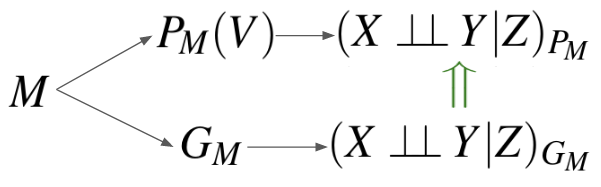
\includegraphics[width=.4\linewidth]{pics/my_own/dsep_Markov_flow.png}
\caption{The green arrow is the directed global Markov property (validity of $d$-separation) when $M$ has a unique solution \color{red}(TODO: check this)\color{black}. The converse of the green arrow is $d$-faithfulness.}
\label{fig:dsep-Markov-flow}
\end{figure}

\subsection{counterexample}

For an illustration of how d-spearation may not hold for cyclic SCMs, consider the following example from \cite{Acyclification} (and further discussed in \cite{Foundations}).

\begin{example}[Counterexample: Loss of d-separation validity]
\label{counter}

Consider the SCM $M=(\mathbf{U},\mathbf{V},F,P(\mathbf{U}))$ with $\mathbf{u}=[u_1,u_2,u_3,u_4]\in \R^4$, $\mathbf{v}=[x_1,x_2,x_3,x_4]\in\R^4$, where $F$ is defined component-wise by
\[
f_1(\mathbf{v},\mathbf{u}) = u_1, \quad f_2(\mathbf{v},\mathbf{u}) = u_2, \quad
f_2(\mathbf{v},\mathbf{u}) = x_1x_4+u_3, \quad f_4(\mathbf{v},\mathbf{u}) = x_2x_3+u_4 
\]
and $P(\mathbf{U})$ is the standard-normal distribution on $\R^4$. The causal graph $G_M$ is shown in Figure \ref{fig:acyclification} (left). For every equilibrium of $M$, the induced observational distribution $P_M(\mathbf{V})$ satisfies $(X_1 \nCI X_2 \mid X_3,X_4)_{P_M}$.
However, $X_1$ and $X_2$ are d-separated given $\{X_3,X_4\}$ in the causal graph; that is, $(X_1 \CI X_2 \mid X_3,X_4)_{G_M}$. 
Hence, the global directed Markov property does not hold for $M$.
\end{example}

\begin{figure}
\centering
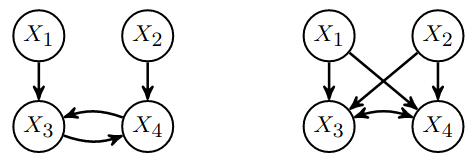
\includegraphics[width=.4\linewidth]{pics/cited/acyclification_Foundations.png}
\caption{The causal graph of Example \ref{counter} (left) and its acyclification (right). Source: \cite{Foundations}}
\label{fig:acyclification}
\end{figure}

When d-separation is not valid (the directed global Markov property does not hold), it may be that a weaker condition is satisfied. $\sigma$-separation is an extension of $d$-separation, which works by applying d-separation to the acyclification of the original graph (see Figure \ref{fig:acyclification} (right) for the acyclicification of Example \ref{counter}). $\sigma$-separation implies $d$-separation; in other words, the general directed global Markov propoery is weaker than the directed global Markov property. The relationship between these two Markov properties can be seen in Figure \ref{fig:inputs-outputs}.

\begin{figure}
\centering
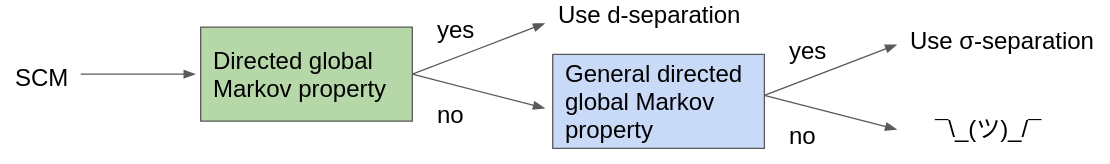
\includegraphics[width=.8\linewidth]{pics/my_own/inputs_outputs.png}
\caption{Relationship between d-separation and $\sigma$-separation.}
\label{fig:inputs-outputs}
\end{figure}

Acyclic SCMs, discrete SCMs (with ancestrally unique solvability), and linear SCMs (with nontrivial dependancies and postive measure) are known to satisfy the directed global Markov property \cite{MarkovCyclesLatent}. On the other hand, simple SCMs are known to satisfy the general directed global Markov property \cite{Foundations}. 

It seems reasonable that nonlinear SCMs which are asymptotically equivalent to linear SCMs should also satisfy the directed global Markov property (subject to the same restrictions of non-trivial dependancies and positive measure), and thus be able to read off conditional independancies from the graph via d-separation.
I conjecture that intrinsically-stable SCMs (a class of cyclic, nonlinear, continuous-domained SCMs) are precisely this class of SCMs.

\begin{problem}[Intrinsic SCMs and d-separation: Observational]
\label{prob:obs}

Prove whether the observational distribution of intrinsically-stable SCMs satisfy the directed global Markov property: that is, whether every conditional independance read-off by d-separation in the causal graph $G_M$ holds in the observational distribution $P_M(V)$.

Inputs/Outputs: Expressed by the green implication in Figure \ref{fig:dsep-Markov-flow}.
\end{problem}

(Admittedly it seems awfully convienent that a topic I studied for over 4 years (undergradate, Master's, and a bit thereafter) happens to be the right tool for the job. However, I think intrinsic SCMs can stand on their own merits):

Considered from a dynamical-systems perspective, intrinsic-SCMs have a number of promising properties relevant to causality. They have a unique equilibrium, so the potential response function of the SCM will be well-defined. They `behave’ like linear systems: they are asymptotically bounded by the dynamics of a linear system, and share the same equilibria if subject to the same forcing factor (exogenous distribution). Intuitively speaking, this means that we can go to linear-world, prove things about the system there, and the results will still hold in nonlinear-world. Furthermore, intrinsically-stable systems are quite general: they only require Lipschitz-continuity, and the domain to be a product of metric spaces (which could be something nice like $\R^4$, or something abstract like language and shapes). If a general domain like metric spaces is used, the linearization uses the metrics to map to the real numbers: in this way the domain is simplified as well.

Of particular interest for causality, intrinsically-stable systems derive their name because they are closed under a surprising number of structural transformations; that is, the resulting system will still be intrinsically-stable, and often (if applicable) the equilibria will be preserved. Some of the transformations that come to mind are: 1. lengthening of paths (i.e. through time-delays), 2. collapsing portions of the graph, 3. duplicating portions of the graph (called specialization), 4. time-varying structural switching, and 5. any and all isospectral transformations (transformations which preserve the eigenvalues of the system).

Given these properties of intrinsic-SCMs, a negative result for Problem \ref{prob:obs} becomes even more interesting. Since intrinsically-stable SCMs are asymptotically equivalent to linear SCMs, if d-separation holds for the linear but not the nonlinear SCM, this would indicate that something more than the equilibria of a cyclic SCM is needed to determine the vaidity of d-seperation. 

\color{red} the previous two paragraphs are a great place to cite intrinsic papers \color{black}

\section{Literature Review}

intrinsic stability!

Intrinsic SCMs contain the space acyclic SCMs (so long as we tweak the definition slightly)
I conjecture that intrinsic SCMs are a subset of simple SCMs

\begin{figure}
\centering

\includegraphics[width=.6\linewidth]{pics/my_own/set_inclusion.png}
\caption{Conjectured set-inclusion relation of the class of intrinsically-stable SCMs relative to other classes of cyclic SCMs. \color{red}Move to be first figure?\color{black}}
\label{fig:set-inclusion}
\end{figure}

\subsection{Frameworks for cyclic causality}
\begin{itemize}
  \item `Foundations' \color{blue} (1 slide)\color{black}
  \begin{itemize}
    \item space inclusion diagram (int. stable between acyclic and simple)
  \end{itemize}

  \item Settable Systems \color{blue} (1 slide)\color{black}
  \begin{itemize}
    \item 
  \end{itemize}
\end{itemize}

\subsection{This problem specifically}
\begin{itemize}
  \item Foundations
  \begin{itemize}
    \item 
  \end{itemize}

  \item Markov Paper?
  \begin{itemize}
    \item 
  \end{itemize}

  \item Linear paper?
  \begin{itemize}
    \item 
  \end{itemize}
\end{itemize}


\section{Preliminary Results}
\subsection{Numerics}

Consider again Example \ref{counter}, the counterexample popular in the literature. If we restrict the domain of the exoenous variables to $\mathbf{u}=\in [-0.5,0.5]^4$ (which we may do by discarding any samples outside of this range), the resulting SCM is intrinsically-stable. Hence, if Problem \ref{prob:obs} resolves in the affirmative, we should observe that the observational distribution of the restricted-domain SCM should have the conditional independence of $(X_1 \CI X_2 \mid X_3,X_4)_{P_M}$, matching the independence $(X_1 \CI X_2 \mid X_3,X_4)_{G_M}$ computed by d-separation from the graph.

The results of this test are shown in Figure \ref{fig:counterexample_domain_restriction}. In order to test the conditional independence numerically over a continous domain, the python package \verb|fcit| was used \cite{fcit}. The resulting p-values are distributed roughly uniformly on $[0,1]$, consistent with an \verb|fcit| result of conditional independence.

\begin{figure}
\centering
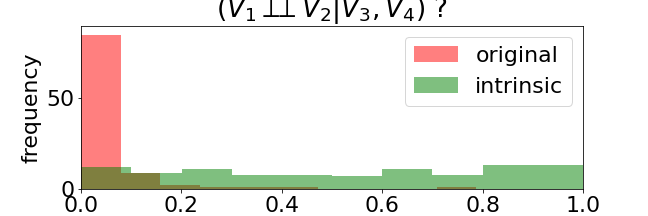
\includegraphics[width=.5\linewidth]{pics/my_own/counterexample_domain_restriction.png}
\caption{The counterexample discussed in \cite{Acyclification,Foundations}. Here, conditional indpendence is tested while restricting the exogenous variables to be drawn from a truncated multivariate normal distribution (such that the SCM as a whole is intrinsically stable). The conditional independence identified by d-seperation is now present in the observational distribution.}
\label{fig:counterexample_domain_restriction}
\end{figure}
 
\subsection{Proof sketch for Problem \ref{prob:obs}}

\begin{figure}
\centering
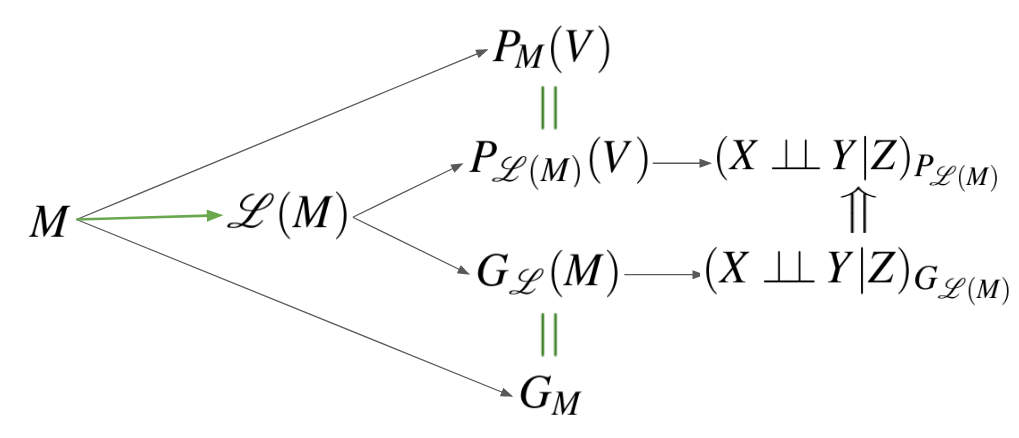
\includegraphics[width=.5\linewidth]{pics/my_own/research_plan_flow.png}
\caption{Conjectured proof sketch, for positive resolution of Problem \ref{prob:obs}.}
\label{fig:research-plan-flow}
\end{figure}

\begin{figure}
\centering
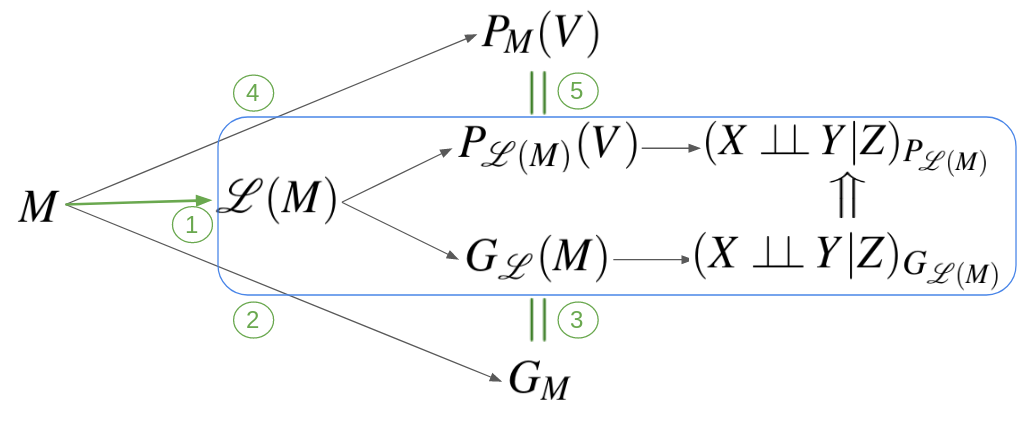
\includegraphics[width=.5\linewidth]{pics/my_own/research_plan_numbered_boxed.png}
\caption{Identical as Figure \ref{fig:research-plan-flow}, but with helpful labels of the conjectured relations. Note that the portion contained within the blue box simply expresses that the associated linear SCM $\mathcal{L}(M)$ satisfies the directed global Markov property (Figure \ref{fig:dsep-Markov-flow}).}
\label{fig:research_plan_numbered_boxed}
\end{figure}

My research strategy for proving the affirmative of Problem \ref{prob:obs}, comprises of two parts (see Figure \ref{fig:research-plan-flow}): First, relate $M$ to a linear SCM $\mathcal{L}(M)$ which satisfies the directed global Markov property. Secondly, show that $M$ and $\mathcal{L}(M)$ respect the same graph and are observationally equivalent.

This can be broken down into greater detail via Figure \ref{fig:research_plan_numbered_boxed}. Each of these parts (with a rough proof sketch) are described below:

\begin{enumerate}
  \item $M\rightarrow \mathcal{L}(M)$: Show that for every intrinsically-stable $M$, there exists a linear SCM $\mathcal{L}(M)$ which satisfies the directed global Markov property (the blue box).
  \item $M\rightarrow G_M$: Always possible by definition, I believe.
  \item $G_M = G_{\mathcal{L}(M)}$: Show that for every node, the parents are preserved (according to \cite{Foundations}'s definition of parents: see Appendix \ref{foundations-material}).
  \item $M \rightarrow P_M(V)$: Show that if $M$ is intrinsically stable, it is uniquely solvable.
  \item $P_M(V) = P_{\mathcal{L}(M)}(V)$: Translate intrinsic-stability property of $M$ and $\mathcal{L}(M)$ have the same equilibrium solutions, to SCMs. Show that this means they induce the same obs. distributions.
\end{enumerate}

\subsection{Anticipated Implications}

I consider it is worth checking early in one's research whether hypothetical success would itself be ludicrous, even if this means initially high exposure to unverified speculation.
To keep this report appropriately rigorous, however, my speculation about these potential implications is located in Appendix \ref{speculation}.
In a sentence: While I do expect positive resolutions to Problems \ref{prob:obs} and \ref{prob:int} to mean that nonlinear, intrinsic SCMs inherit many of the nice properties of linear cyclic SCMs, I also expect this will not violate the `No Free Lunch' Principle: the resulting linear SCMs will be no easier to use for modeling purposes.

\subsection{Potential (future) Collaborators}

I recently met with both Lewis Hammond (Oxford) and Christian Kroer (Columbia, IOER department). Both are very interested in `game theory + causality', which I find the most compelling motivator for cyclic causality research. To the extent that nonlinear, cyclic SCMs are `locally intrinsic' (as Example \ref{counter} was shown to be here) there may be some valuable collaborations to be had. For now, I'll just keep occasional dialogue with them to see what arises.

% %%%%%%%%%%%%%%%%%%%%%%%%%%%%%%%%%%%%%%%%%%%%%%%%%%%%%%%%%%%%%%%%%%%%%%%%%%%%%%%%%%%%%%%

% \section{Problem Formulation}

% % \color{red} TODO: \color{black}

% Current Conjectures
% \begin{itemize}
%   \item Conjecture 1: I can replace “linear” in Theorem 6.3 part 1(c) with “intrinsically stable”
%   \begin{itemize}
%     \item Which means d-separation is guaranteed to hold in an broad non-linear, cyclic setting
%     \item See Markov Properties for Graphical Models with Cycles and Latent Variables: In [Spi94] an example of a directed graph with cycles and corresponding non-linear structural equations was given such that certain expected conditional independence relations were missing. This showed that the structural equations property (SEP) i.g. does not imply the directed global Markov property (dGMP) in the presence of cycles. Another example will be given in 3.8.6. So the following two questions arose…
%     \item Is this the same as the following quote from Causal Modeling of Dynamical Systems? ...Given that steady SDCMs for which all solutions equilibrate give rise to SCMs at equilibrium, the inverse problem becomes interesting as well: given an SCM, can we find an SDCM (with non-trivial dynamics) that equilibrates to this SCM and for which all solutions equilibrate? This question was answered affirmatively for a certain class of linear simple SCMs with additional constraints on the parameters by leveraging existing results from linear systems theory. We speculate that this result can be further generalized to allow for non-linearity.
%   \end{itemize}

%   \item Conjecture 2: Every intrinsically-stable SCM is simple.
%   \begin{itemize}
%     \item Conjecture 2a: No intrinsically-stable SCM has self-cycles (by the definition provided in this paper).
%   \end{itemize}

%   \item Conjecture 3: For all simple SCMs, there is an intrinsically-stable SCM equivalent to it.
%   \begin{itemize}
%     \item So even though the set of “intrinsically stable SCMs” is contained within the set of “simple SCMs”, it’s broad enough to capture everything we care about.
%     \item (I expect this won’t hold in general, but I do expect it to hold for all continuous, smooth, or otherwise “nice” SCMs; aka all the ones practitioners would actually care about)
%   \end{itemize}

%   \item Conjecture 4: Equivalence is preserved under isospectral transformation.
%   \begin{itemize}
%     \item This means we can use any isospectral transformation to change the graph into one that is easier to analyze.
%   \end{itemize}

%   \item I think the usefulness of Conjectures 2 and 3 are dependent on the validity of Conjecture 1. 
%   \begin{itemize}
%     \item Conjecture 4 seems less important than Conjecture 1, but may still have independent usefulness.
%   \end{itemize}

%   \item Conjecture 5: Let $M$ be an SCM with differentiable $F$. Let $F_L$ denote the unique minimal Lipchitz mapping of $F$. Then for each $v_i$, the parents (as defined in Foundations) of $v_i$ w.r.t. $F$ are identical to the parents w.r.t. $F_L$.
%   \begin{itemize}
%     \item I think a corrollary of this would be that the graphs will be identical.
%     \item I think this would be a useful lemma for showing independancies hold (so, for the d-separation result).
%   \end{itemize}

%   \item 
%   \begin{itemize}
%     \item 
%   \end{itemize}

%   \item 
%   \begin{itemize}
%     \item 
%   \end{itemize}
% \end{itemize}


% Extending d-separation to intrinsically-stable models
% \begin{itemize}
%   \item Conjecture 5: Let $M$ be an SCM with differentiable $F$. Let $F_L$ denote the unique minimal Lipchitz mapping of $F$. Then for each $v_i$, the parents (as defined in Foundations) of $v_i$ w.r.t. $F$ are identical to the parents w.r.t. $F_L$.
%   \begin{itemize}
%     \item I think a corrollary of this would be that the graphs will be identical.
%     \item I think this would be a useful lemma for showing independancies hold (so, for the d-separation result).
%   \end{itemize}

%   \item it's plausable that the "Lipschitz linearization preserves equivalences" conjecture could be useful for d-separation
%   \begin{itemize}
%     \item although it's a little fuzzy to me how. Going between different representations, perturbing on a set of measure 0, ....
%     \item Conjecture: If $M_1$ and $M_2$ have the same observational graph and distribution, and the global markov property holds on $M_1$, then it holds on $M_2$, at least for that graph/distribution. (not necessarily subgraphs).
%     \item I need to know what the global Markov property says!
%   \end{itemize}
  
%   \item The core of the matter:
%   \begin{itemize}
%     \item What even is the markov property that I need to show?
%     \item Can I locate the proof for the linear case?
%   \end{itemize}
% \end{itemize}

% \subsection{Markov notes from Foundations, appendix}
% \begin{itemize}
%   \item They claim it serves as a good intro to the more extensive paper/literature

%   \item The directed global Markov property
%   \begin{itemize}
%     \item `The directed global Markov property associates a conditional independence relation in the observational distribution of the SCM to each d-separation entailed by the graph.'
%     \item They use a formulation of d-separation that generalizes d-separation for DAGs, m-separation for ADMGs, and mDAGs.
%     \item The definition of collider is as expected (the same as for m-separation).
%     \item 
%   \end{itemize}

%   \item 
%   \begin{itemize}
%     \item 
%   \end{itemize}

%   \item 
%   \begin{itemize}
%     \item 
%   \end{itemize}
% \end{itemize}

% \subsection{Problem statement}
% \begin{itemize}
%   \item Don't mention intrinsically-stable models in the problem statement: it is merely the solution which solves the problem.
%   \item Investigate whether 
% \end{itemize}




%%%%%%%%%%%%%%%%%%%%%%%%%%%%%%%%%%%%%%%%%%%%%%%%%%%%%%%%%%%%%%%%%%%%%%%%%%%%%%%%%%%%%%%

% \section{Lit. Review: Foundations \cite{Foundations}}

% `Foundations of structural causal models with cycles and latent variables' by Bongers et. al. \cite{Foundations} outlines a modeling framework for cyclic SCMs that is quite similar to Pearl's framework for acyclic SCMs.
% Cycles are incorperated simply by allowing the function $F$ of the SCM $M=(U,V,F,P(U))$ to be dependent on any variables in $U\cup V$.
% % While technically SCMs without a unique fixed point are can still be expressed within the framework, the authors focus primarily on situations where a unique fixed point exists.
% This paper focuses on atomic interventions (which they call `perfect interventions').

% Previously in the literature, it had already been established that many nice properties of acyclic SCMs can be lost once cycles are allowed. For example, 1. Potential response functions may not exist; 2. The observational / interventional / counterfactual distributions may not exist, or if they do, they may not be unique; 3. Marginalizing over variables may not be possible, or sensible; 4. d-separation may not hold (aka. the `directed global Markov property') 5. $\sigma$-separation may not hold (aka. the `general directed global Markov property'; a weaker form of d-separation); 6. the induced causal graph may not be consistent with the SCM's causal semantics. 

% There are several aspects of this framework which contrast with Pearl \cite{pearl_2009}.
% The authors emphasize almost-everywhere equivalence, with respect to the observational, interventional, and counterfactual distributions, or structural functions themselves. This empahsis implicitly impacts their definitions. For example, and notably, the definition of a variable's `parents' excludes any trivial dependancies: node $k$ is a parent of $i$ only if a measurable function cannot be found which does not depend on $k$ and almost-everywhere matches the structural function for node $i$. While this definition is semantically useful (we only say there's a parent if there's a dependence that really can't be ignored) it can be slightly confusing: for example, consider the two-node linear system of $x_1 = f_1(x_1,x_2)=0.5x_1+0.1x_2$ and $x_2 = f_2(x_1,x_2)=0.1x_1+0.5x_2$. According to the definitions of \cite{Foundations}, $x_1$ and $x_2$ are both parents of each other, yet no self-cycles exist, because there exists an SCM which is asymptotically equivalent without self-cycles. (This property of linear systems will be discussed further in Section \ref{section:learninglinear}; see Figure \ref{fig:SelfCycles}).

% Besides presenting unifying notation and sythesizing a cohesive review of much of the work on cyclic SCMs, the authors also present their own significant contribution: simple SCMs. Simple SCMs are SCMs which are uniquely solvable with respect to every subset of variables. Intuitively, this means that every submodel has a unique fixed point (so the potential response function is well-defined for each submodel). This is a sufficient condition for the observational, interventional, and counterfactual distributions to exist and be unique. Furthermore, simple SCMs satisfy a weaker form of the d-sepearation criterion, called $\sigma$-separation (a.k.a. the general directed global Markov property). Simple SCMs are closed under marginalization, and the marginalization respects the latent projection (that is, the causal sematics of the causal diagram's subgraph match the structure of the submodel of the SCM).
% The relationship of simple SCMs to previous classes of cyclic SCMs explored in the literature is shown in Figure \ref{fig:CylicClasses}. 
% (For the sake of this review, it suffices to say that modular SCMs are a class of cyclic SCMs which contain the class of simple SCMs; causal constraint models, CCMs, are a generalization of SCMs which is expressive but lacks a satisfying graphical representation).
% \begin{figure}
% \centering
% 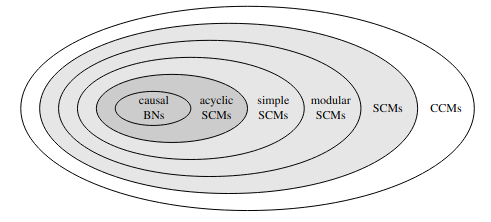
\includegraphics[width=.6\linewidth]{pics/cyclic_classes.png}
% \caption{An inclusion diagram of various modeling frameworks for cyclic SCMs. Source\cite{Foundations}}
% \label{fig:CylicClasses}
% \end{figure}

% %%%%%%%%%%%%%%%%%%%%%%%%%%%%%%%%%%%%%%%%%%%%%%%%%%%%%%%%%%%%%%%%%%%%%%%%%%%%%%%%%%%%%%%

% \color{blue} 90 minutes (timed show-up) to provide a workable review of the paper. Then I copy it over to the report. \color{black}

% % Answer all of the following questions within 60 minutes total. After that, spend 10 minutes reorganizing them and smoothing it into a cohesive review. The final 5 minutes are just a breather :) .

% \section{Lit. Review: Learning Linear \cite{LearningLinear}} \label{section:learninglinear}
% \color{blue} In your own words, what are the most important aspects of the framework used in `Learning Linear'? \color{black}
% \begin{itemize}
%   \item 
% \end{itemize}

% \color{blue} In what ways does this framework differ from Pearl? Were there any surprises you encountered while reading? What confusions did you have that got cleared up? [TODO: cite Pearl]. \color{black}
% \begin{itemize}
%   \item 
% \end{itemize}

% \color{blue} What are the most significant results from `Learning Linear'? \color{black}
% \begin{itemize}
%   \item 
% \end{itemize}

% \color{blue} What sort of previous work is `Learning Linear' building on? \color{black}
% \begin{itemize}
%   \item 
% \end{itemize}

% \begin{figure}
% \centering
% 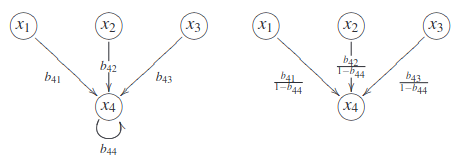
\includegraphics[width=.6\linewidth]{pics/self_cycles.png}
% \caption{Source: \cite{LearningLinear}}
% \label{fig:SelfCycles}
% \end{figure}

% \color{red} TODO: \color{black}


% %%%%%%%%%%%%%%%%%%%%%%%%%%%%%%%%%%%%%%%%%%%%%%%%%%%%%%%%%%%%%%%%%%%%%%%%%%%%%%%%%%%%%%%

% \section{Lit. Review: Settable Systems \cite{White&Chalak}}
% \begin{itemize}
%   \item 
% \end{itemize}

% %%%%%%%%%%%%%%%%%%%%%%%%%%%%%%%%%%%%%%%%%%%%%%%%%%%%%%%%%%%%%%%%%%%%%%%%%%%%%%%%%%%%%%%

% \section{Lit. Review: Game Incomplete \cite{GameIncomplete}}
% \begin{itemize}
%   \item 
% \end{itemize}

% %%%%%%%%%%%%%%%%%%%%%%%%%%%%%%%%%%%%%%%%%%%%%%%%%%%%%%%%%%%%%%%%%%%%%%%%%%%%%%%%%%%%%%%

% \section{Lit. Review: Markov Properties \cite{MarkovCyclesLatent}}
% \begin{itemize}
%   \item 
% \end{itemize}

% %%%%%%%%%%%%%%%%%%%%%%%%%%%%%%%%%%%%%%%%%%%%%%%%%%%%%%%%%%%%%%%%%%%%%%%%%%%%%%%%%%%%%%%

% \section{Lit. Review: Dynamical Systems \cite{DynamicalSystems}}
% \begin{itemize}
%   \item 
% \end{itemize}

%%%%%%%%%%%%%%%%%%%%%%%%%%%%%%%%%%%%%%%%%%%%%%%%%%%%%%%%%%%%%%%%%%%%%%%%%%%%%%%%%%%%%%%

% pdflatex main
% bibtex main
% pdflatex main
% pdflatex main

\bibliographystyle{plain}
\bibliography{refs}

\section{Appendix: Musings Beyond Observational d-seperation}

\subsection{d-seperation and Interventional Distributions} \label{speculation}

I’m very confident that the space of intrinsic SCMs is closed under interventions (if you intervene on an intrinsic SCM, the resulting SCM is also intrinsic).
I’m also confident that the operations of atomic intervention $M\rightarrow M_x$ and linearization $M\rightarrow \mathcal{L}(M)$ commute for intrinsic SCMs.
Thus, if Problem \ref{prob:obs} resolves in the affirmative, I conjecture it should be straightforward to demonstrate (atomic) interventional equivalence between a nonlinear, intrinsic SCM and its associated linear SCM $\mathcal{L}(M)$.

\begin{problem}[Intrinsic SCMs and d-separation: Interventional]
\label{prob:int}

Prove whether the interventional distribution of intrinsically-stable SCMs satisfy the directed global Markov property: that is, whether every conditional independance read-off by d-separation in the causal graph $(G_M)_{\overline{X}}$ holds in the interventional distribution $P_{M_x}(V)$.
\end{problem}

Note the order of operations for $(G_M)_{\overline{X}}$: first we generate the causal graph of $M$, then intervene with an atomic intervention on that graph. This is in contrast to $P_{M_x}(V)$, where we first perform an atomic structural intervention on $M$, then generate the distribution of this new SCM.

If Problem \ref{prob:int} answers in the affirmative, I believe it follows that the do-calculus is valid for intrinsic SCMs.

\subsection{d-seperation and Counterfactual distributions}

I also confidently conjecture that (if Problem \ref{prob:obs} resolves positively) intrinsic SCMs are also closed under the “mirror” transformation.
(The mirror operation is useful for defining cyclic counterfactuals: you construct a `twin SCM' using the twin network method). 
This operation, if I understand correctly, should merely reduce to the duplication of a strongly connected component, but othewise leave strongly connected components unchanged. Since intrinsic-stability is based on a spectral criteria, one can without loss of generality simply consider each strongly connected component of the system independently. (Indeed, almost all my remaining uncertainty derives from wondering whether I've missed some subtle-yet-crucial detail in the definitions of cyclic SCMs).

\begin{problem}[Intrinsic SCMs and d-separation: Counterfactual]
\label{prob:count}

Prove whether the counterfactual distribution of intrinsically-stable SCMs satisfy the directed global Markov property: that is, whether every conditional independance read-off by d-separation in the twin network holds in the corresponding counterfactual distribution of the twin SCM.
\end{problem}

If Problem \ref{prob:count} resolves positively, then this would mean that the $M$ and $\mathcal{L}(M)$ are not merely observationally or interventionally equivalent, but \emph{counterfactually equivalent}. (However, they are precluded from being \emph{structurally equivalent} according to the definition in \cite{Foundations}, since this requires not only almost-everywhere equivalence of equilibrium solutions, but of the transition functions themselves.)

I do not expect this counterfactual equivalence (should it actually hold) to violate the `No Free Lunch' principle.
The counterfactual equivalence of an intrinsic SCM $M$ with a linear SCM $\mathcal{L}(M)$ may do little more than imply that nice properties (like d-seperation) are valid for $M$, as far as modeling is concerned, because I expect that the complexity of $F_M$'s nonlinearity simply gets pushed into the linear SCM's exogenous distribution $P_{\mathcal{L}(M)}(U)$.

\section{Appendix: Relevant Definitions for Cyclic SCMs}\label{foundations-material}
The following definitions are copied verbatim from \cite{Foundations}, and provided here only for ease of reference. Consequently they differ somewhat from the notation of this report.

\centering
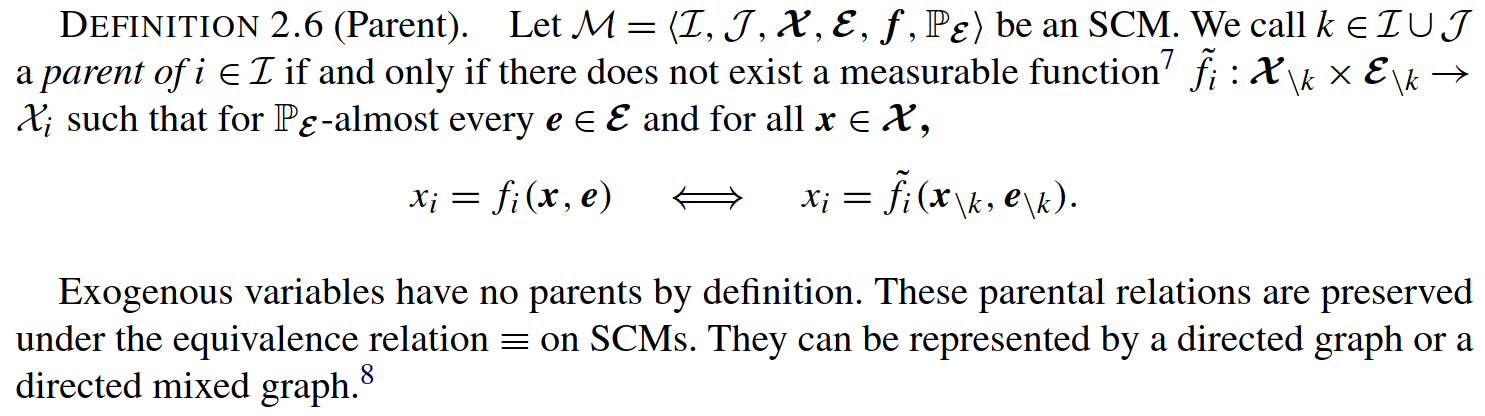
\includegraphics[width=.8\linewidth]{pics/cited/parents_Foundations.png}

\centering
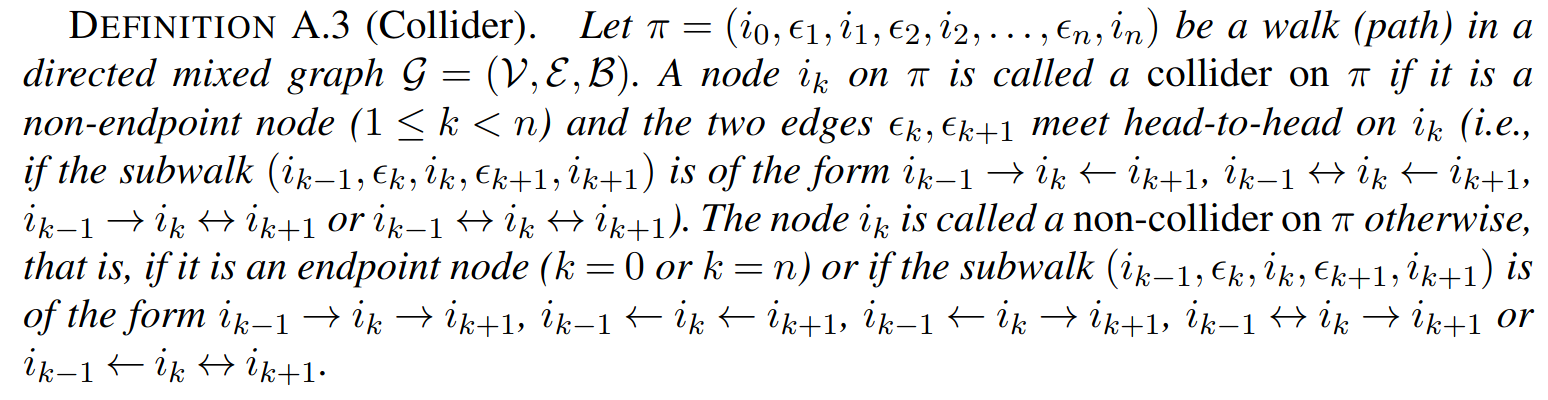
\includegraphics[width=.8\linewidth]{pics/cited/collider_Foundations.png}

\centering
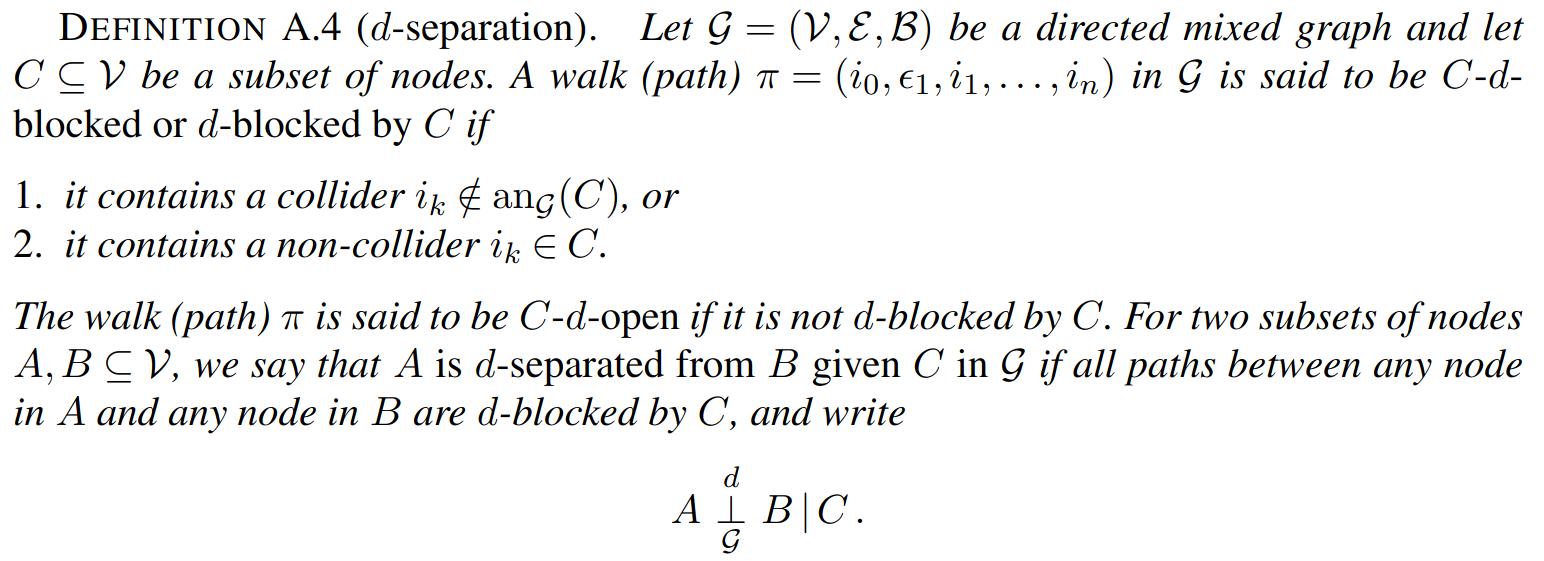
\includegraphics[width=.8\linewidth]{pics/cited/d-separation_Foundations.png}

\centering
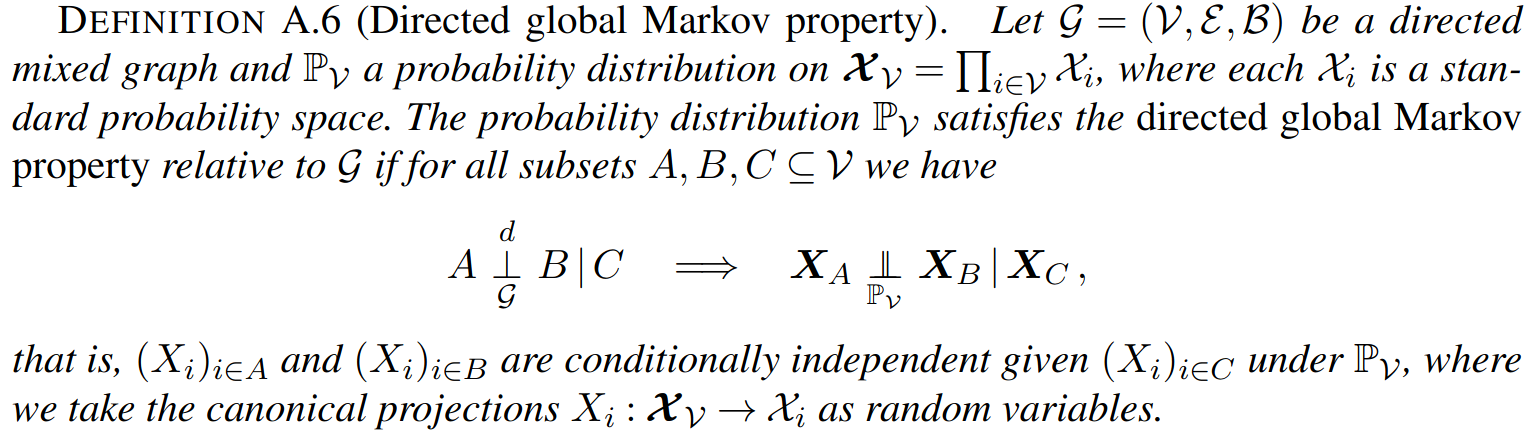
\includegraphics[width=.8\linewidth]{pics/cited/directed_global_Markov_Foundations.png}

\end{document}
